\chapter{Simulator Design and Implementation}

This chapter describes the design and implementation of PBTSim (Priority Based Traffic Simulator), a software package to allow for simulation and evaluation of priority based traffic control. To produce a representative comparison with existing SCATS-based systems, creating a realistic simulation environment was a key implementation challenge, and a primary objective of this project. The outcomes discussed in this chapter are:

\begin{itemize}
\item using the open-source software package MovSim as a framework for implementation of PBTSim,
\item extending the MovSim package within PBTSim to support development of the PBTC control algorithm and allowing for multiple control algorithms to be developed and evaluated,
\item development of a parser for SCATS log files, to allow for traffic flow rates and traffic signal phase timings to be read from a SCATS log file and used in simulation.
\end{itemize}

\section{Simulation Platform}

A primary challenge of measuring and evaluating performance of an adaptive traffic control system is the requirement to simulate realistic traffic conditions with sufficiently measurable results. Software for simulating traffic control methods is typically developed by vendors of a particular system and as such is proprietary and not available for research. Because of this, an open-source tool called MovSim is used as a framework for development and evaluation within this project. MovSim (Multi-model Open-source Vehicular-traffic Simulator) is an open-source, Java-based traffic simulator implementing multiple time-continuous, car-following traffic models designed for investigating traffic dynamics; currently under active development. MovSim implements a wide range of configurable vehicle-following, acceleration, and lane changing models that determine individual vehicle movement within the simulation \cite{movsim,kesting2013traffic}.

\begin{figure}[]
\centering
	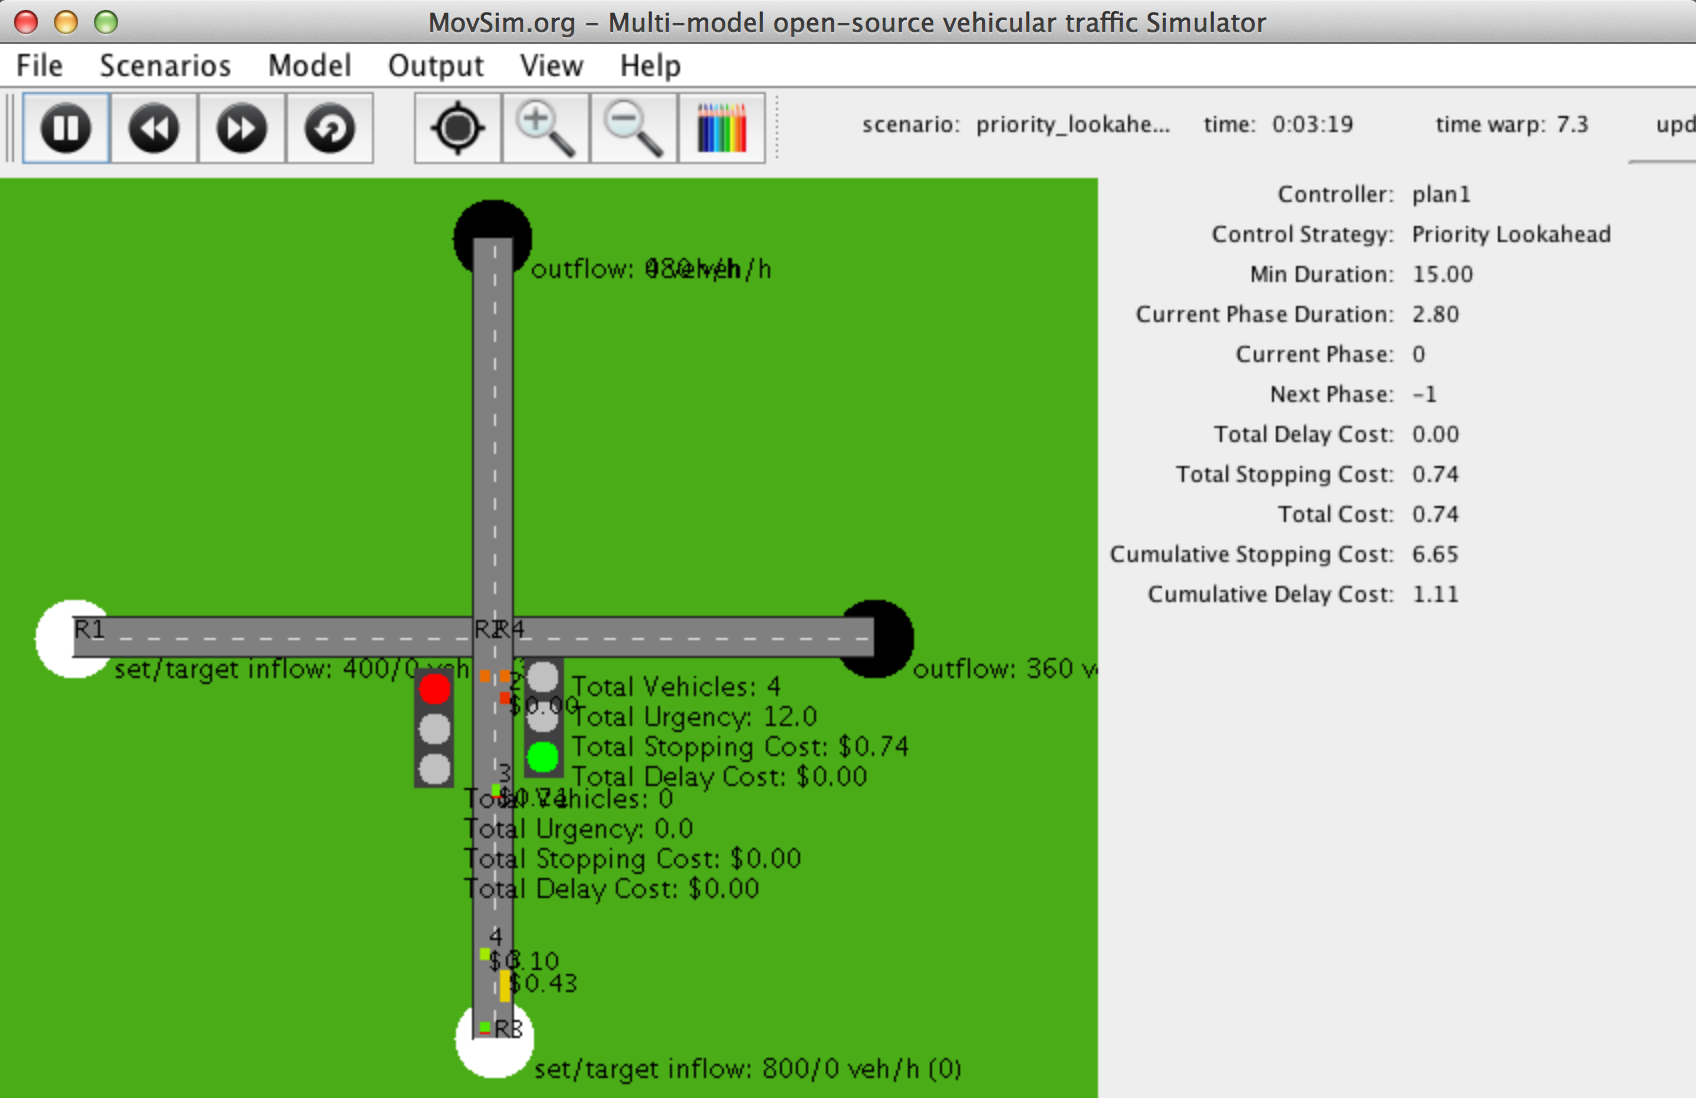
\includegraphics[scale=0.35]{movsim-interface.png}
	\caption[A screenshot of the PBTSim user interface showing an example intersection.]{ A screenshot of the PBTSim Graphical User Interface running a simulation of the four-way intersection scenario used during design and evaluation of the PBTC control system. }
\label{pbtsim-interface}
\end{figure}

All software artefacts produced during this project were implemented within a fork of the MovSim project, which we have named PBTSim (Priority Based Traffic Simulator). PBTSim is a software application that allows for simulation and evaluation of traffic control methods based on the vehicle priority model described in Chapter \ref{chapter:design}. Figure \ref{pbtsim-interface} shows a screenshot of the Graphical User Interface (GUI) of the PBTSim application. While priority based traffic model features specific to this project are maintained in PBTSim, general purpose features and improvements to the MovSim project have been offered back to the original MovSim repository as potential improvements to be considered by the maintaining authors. 

Limitations of using the MovSim project as a base simulation tool for the PBTSim include lack of support for bi-directional traffic flow and turning behaviour at intersections, both requirements for accurate modeling of a real world road network. Both of these features are areas of future development for the MovSim project. The sophisticated traffic modeling capabilities of the MovSim application, have outweighed these limitations during development of the PBTC system.

\section{Phase Model}

MovSim allows for customisable phases to be configured in the project description file, an XML document describing user-defined settings for traffic composition, simulation variables, and traffic controller plans. Traffic controller phases can be defined in the project description file as an ordered list, with each phase including a list of the state (green, amber, or red) for each traffic light for a given controller. 


%1
The phase model used in most modern traffic control systems is a finite state machine consisting of a set of states for each traffic light connected to the controller, with a set of constraints that define valid states and allowed transitions between states. The basic phase model implemented within the MovSim project follows this approach, however MovSim requires a distinct phase for each period of intergreen time. For example, Figure \ref{movsimphasediagram} shows how a two-phase intersection requires a minimum of six configured phases to incorporate intergreen and all-red periods of operation using the MovSim model. This model requires more design and configuration effort, and does not enforce intergreen periods of operation between two active phases.

\begin{figure}[]
\centering
	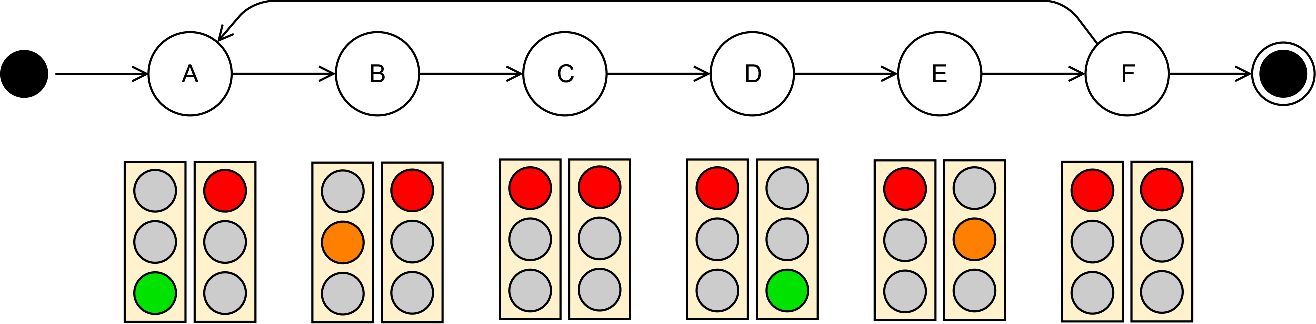
\includegraphics[scale=0.60]{movsim-phasesv2.pdf}
	\caption[A diagram of a set of phase states for a two-phase intersection within the MovSim simulator.]{ A diagram of the available phase states and transitions of a ``two-phase'' intersection configuration within the MovSim simulator. MovSim requires intergreen and all-red periods to be configured as individual phases and does not allow a simple mechanism for skipping, repeating, or alternating the order of configured phases. }
\label{movsimphasediagram}
\end{figure}

To solve this problem, a new phase model was developed for the PBTSim simulator during this project. The developed model is similar to the phase model used by SCATS, where each phase includes a fixed number of seconds as minimum time, maximum time, and intergreen time. It is assumed that during an intergreen period any traffic lights currently displaying a green signal transition to yellow, and all others remain the same. Using this model, the need for additional phases to explicitly define intergreen periods of operation is redundant and the PBTSim simulator enforces intergreen constraints between active phases. Figure \ref{pbtsim-phase-diagram} shows a state diagram of the PBTSim representation of the same ``two phase" configuration described in Figure \ref{movsimphasediagram}.

\begin{figure}[]
\centering
	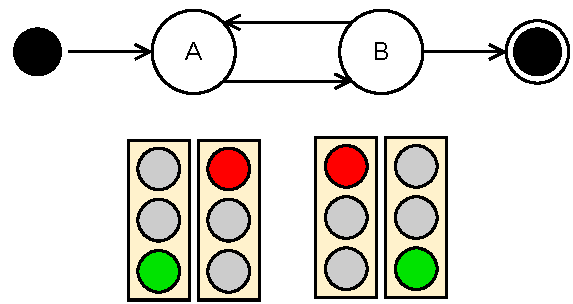
\includegraphics[scale=0.60]{pbtsim-phases.pdf}
	\caption[A diagram of a set of phase states for a two-phase intersection within the PBTSim simulator.]{ A diagram of the available phase states and transitions of a ``two-phase'' configuration within the PBTSim simulator. Intergreen and all-red times are encoded as properties of each phase and the scheduling of these phases is moved to application logic to simplify the phase configuration. }
\label{pbtsim-phase-diagram}
\end{figure}

%2
While appropriate for simple examples and fixed-time phases, the basic MovSim implementation of phase configuration is not appropriate for advanced controller strategies, including the PBTC strategy, where skipping phases with no traffic demand is desirable. It is difficult to express skipping of phases in the MovSim phase model, as there is no clear distinction between an intergreen phase and an ``active'' phase to indicate which phases are allowed to be skipped. For example, skipping the ``next'' phase of a currently active phase will cause the traffic controller to skip the amber phase and change to an all-red phase immediately, rather than the desired behaviour of skipping the next active phase.

The new phase model of PBTSim addresses this problem as intergreen and all-red periods of operation are enforced during transitions between active phases, rather than as phases themselves. As a result, expressing skipped phases or operating phases out of order is greatly simplified. The new phase model developed during this project has been provided to the MovSim authors as a potential improvement.

% good up to here jm 04.10.13

\section{Vehicle Priority Simulation}

Priority based traffic modeling is a concept specific to this project and is not implemented in any form within the MovSim simulator. To allow for implementation of the PBTC control system, PBTSim implements the priority model described in Chapter \ref{chapter:design} for all vehicles, and simulates communication between vehicles and a traffic light controller as required by the PBTC control system.

\subsection{Traffic Composition}

The priority model described in Chapter \ref{chapter:design} assumes that occupants of all vehicles on a road network have an urgency of travel, defined as a discrete integer between one and five. As this is an arbitrary, relative scale of motorist urgency, a model of the distribution of driver urgencies for a given time or particular intersection are unknown and not easily measured. As a result, the distribution of urgency values of traffic within the PBTSim system is estimated using an enumerated probability distribution which assigns an arbitrary probability of occurrence to each urgency value for each class of vehicle within the simulation. Table \ref{urgencydistribution} shows the probability distribution of urgency values for each class of vehicle in the PBTSim system. 

\begin{table}[]
\begin{center}
\begin{tabular}{lrrrrr}
\toprule
 & \multicolumn{5}{c}{Passenger Urgency} \\
 \cmidrule(lr){2-6}
Vehicle Class & 1 & 2 & 3 & 4 & 5 \\
\midrule
Car (Light Vehicle) & 0.2 & 0.25 & 0.395 & 0.15 & 0.005  \\
Bus (Heavy Vehicle) & 0.3 & 0.5 & 0.2 & 0.0 & 0.0 \\
Truck (Heavy Vehicle) & 0.1 & 0.5 & 0.3 & 0.1 & 0.0 \\
\bottomrule
\end{tabular}
\end{center}
\caption{Probability values for an enumerated integer distribution of individual vehicle urgencies. Each urgency value in the range 1--5 is associated with a probability of occurrence for a single vehicle. }
	\label{urgencydistribution}
\end{table}

Probability values are assigned to give a one-sided distribution that assumes there are lower proportions of truly urgent road users than not. Buses and trucks have relatively lower average urgency values compared to passenger cars. This measure is used to reflect that public transport makes no guarantees on arrival time for each single passenger, hence most passengers using public transport allow more time than required to reach their destination and that the majority of freight trucks operate on long inter-city journeys, hence the proportion of time potentially spent waiting in traffic lights in a city is small compared to the relatively long journey time. Alternatives not considered include specifying public service vehicles as high priority with the hope of improving the punctuality of bus services. %cite?

\subsection{Approach Communication}

A requirement of the design of the PBTC control system is that all vehicles approaching an intersection must broadcast their position, physical properties, and required passenger characteristics to a traffic controller. As MovSim was not designed to this specification, a new system of simulated communication between vehicles and traffic controllers was designed for the PBTSim simulator.

Each traffic controller within the simulation maintains a list of broadcasts they have received as a map and each new broadcast replaces any existing broadcast from each unique vehicle. An individual broadcast contains properties required by a controller in order to calculate operational stopping cost and delay cost estimated for each individual vehicle, specifically vehicle weight, speed, acceleration, urgency, number of passengers, and distance to the intersection stop-line. Once a vehicle has cleared the stop-line of an intersection, their broadcast is removed from the traffic controller map. 

In order to ensure that the PBTSim environment is representative of a realistic road network and network infrastructure, efforts are made to ensure that the simulated communication between approaching vehicles and a traffic controller includes consideration of the challenges of a real-world communications network. In a simulated environment, vehicle properties can be broadcast instantly, without network costs or delay; however in reality, network topology and bandwidth limitations are factors that reduce the availability of broadcasts. To introduce consideration of networking latency into PBTSim, a two-second delay is imposed on each broadcast from an individual vehicle. This is not designed to be an accurate representation of network imperfections, but does reflect consideration of these factors.

%An alternative design considered involved allowing delay and stopping costs to be calculated and broadcast by the vehicle itself. This method has the advantage of reducing the amount of calculations that are required to be made by a traffic controller, however this distributed computation is more difficult to implement successfully and there are no guarantees that all vehicles will implement the same cost calculations. This method is also difficult to update if changes to the cost calculations were desired after installation.

\section{Control Strategies}

MovSim includes a basic implementation of traffic control capable of operating an ordered list of traffic light phases defined in the simulation configuration file, however the implementation is limited to fixed-time phase control only, where each phase runs for a predetermined number of seconds before transitioning to the next phase. In order to allow for evaluation of multiple phase control strategies to be tested during simulation, a more sophisticated architecture design was implemented during development of the PBTSim system. 

Changes made to the traffic control architecture of PBTSim during this project were designed to be modular and avoid limiting the scope of future work or potential for implementation changes. Figure \ref{controllerclassdiagram} shows a UML class diagram of the type relationships in the traffic control architecture of PBTSim. ControlStrategy is a Java interface class created in PBTSim which implements the Strategy Pattern, an object-oriented design pattern that allows for dynamic selection of a strategy implementation at runtime \cite{gangof4}. This pattern is well-suited to the design of the control strategy algorithm as new strategies (such as the PBTC control strategy) can be added to the system by implementing the strategy interface and defining their own behaviour. 

The ControlStrategy interface is called by a TrafficLightControlGroup class, which controls the state of lights within the simulator. Methods of the ControlStrategy interface allow a TrafficLightControlGroup to check if conditions for scheduling a phase change have been met and acknowledge the change to the strategy once it has been made. Each concrete implementation of the ControlStrategy class can implement their own conditions and strategies that will trigger a change. This relationship creates a separation of concerns between controlling traffic light state and defining traffic light behaviour, allowing for new behaviours to be easily added independently of all other existing strategies and state machine behaviour.

\begin{figure}[]
\centering
	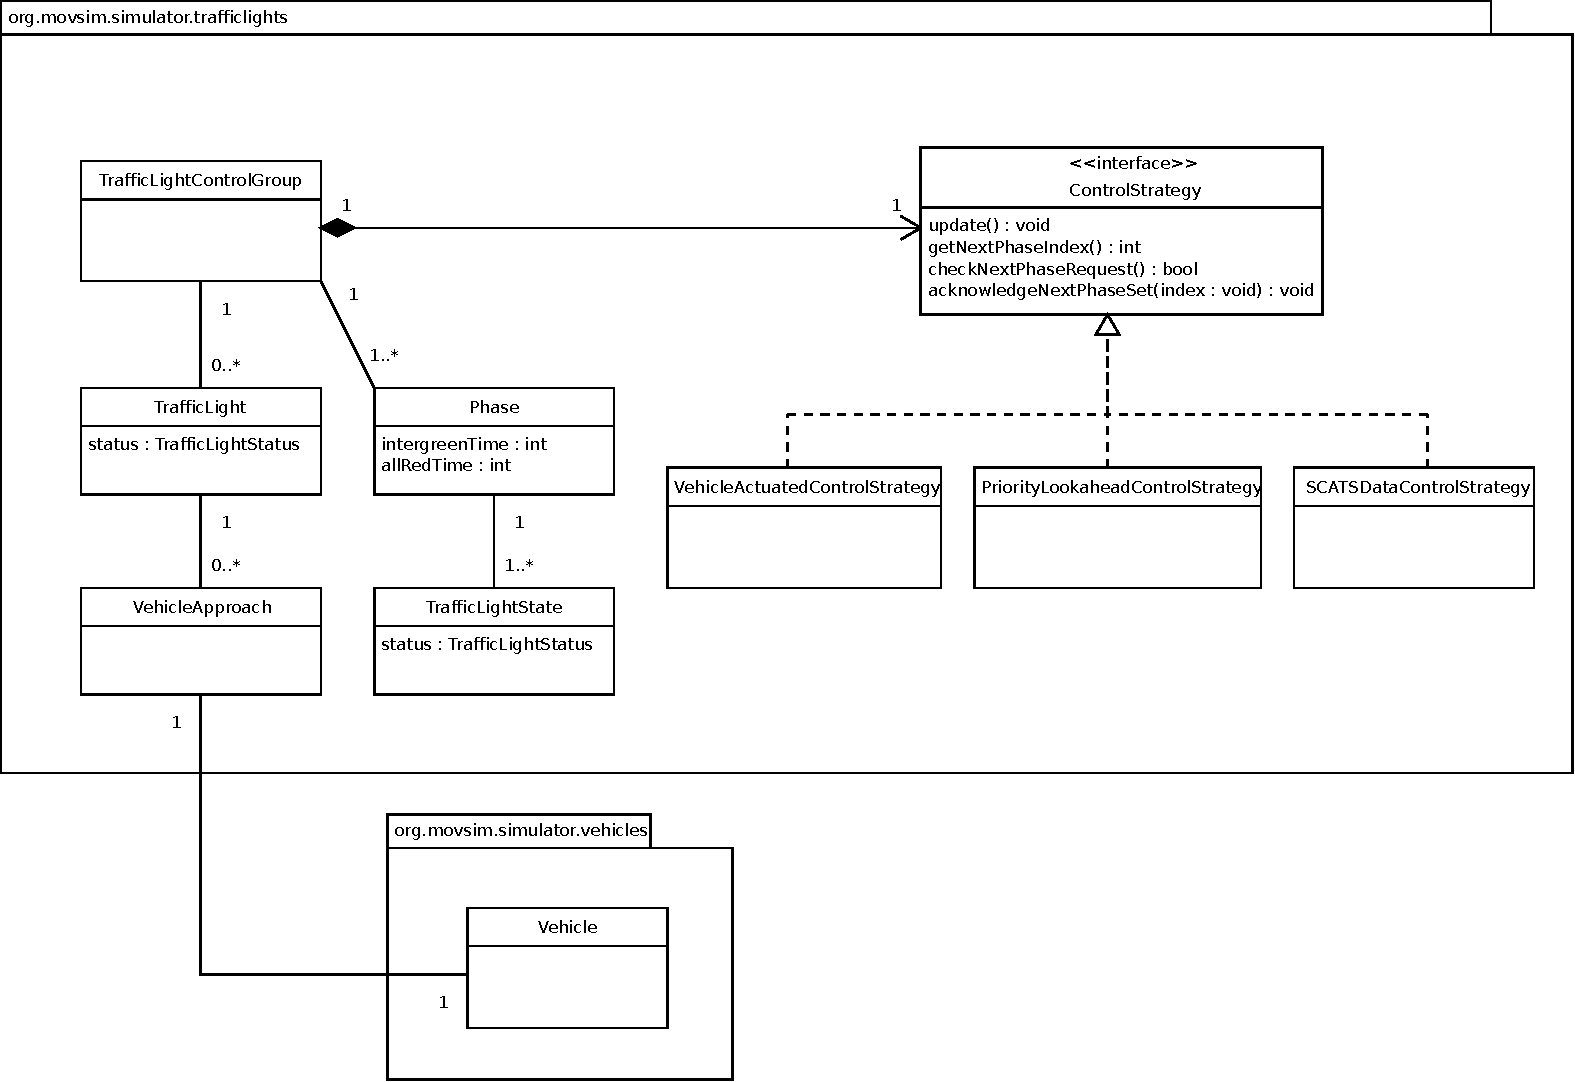
\includegraphics[scale=0.60]{controller_class_diagram.pdf}
	\caption[A UML class diagram of the PBTSim application architecture.]{ A UML class diagram showing the use of the strategy pattern between the TrafficLightControlGroup and ControlStrategy types. ControlStrategy is an interface defining methods required by the TrafficLightControlGroup to change the phase of a set of traffic lights. Three strategies implementing the ControlStrategy interface are shown. Each concrete strategy implementation has a different internal set of conditions to trigger phase changes. }
\label{controllerclassdiagram}
\end{figure}

% good up to here

\section{Design of the PBTC Control Strategy}

The PBTC control algorithm described in Section \ref{sec:PBTCDesign} is designed as a concrete ControlStrategy implementation within PBTSim. The strategy implementation of the PBTC control algorithm consists of two primary phases of operation; approach cost calculation and phase scheduling. 

The PBTC control algorithm implementation is designed to dynamically calculate the sum of the individual estimated delay and operational stopping costs for all of the vehicles on each approaching link of the intersection at each simulator update. The current phase of a PBTC traffic controller operates continuously until the calculated cost of delay on all stopped approaches exceeds than the cost of stopping green approaches, at which point the next phase is allocated and the controller enters the phase change sequence. Once the controller has entered the phase change sequence, it is  committed to changing phases and the lookahead optimisation method is employed to determine whether the phase should change now, or some point in the future, based on the real-time position and state information of vehicles on approaching links. 

% this section is good
\subsection{Lookahead Optimisation}

PBTSim implements the PBTC control algorithm's lookahead features using a map to construct a table of cost values at the end of each phase, once the phase change sequence has been initiated. The lookahead table includes an estimate of the instantaneous change costs for all vehicles known to the PBTC controller at the time the phase change sequence was entered. For each second up to the defined size of the lookahead table, $K$, the PBTC control strategy estimates the cost of changing phases by finding the sum of the cost of stopping, and the cost of delay for the minimum duration of the next phase in the controller sequence for every individual vehicle approaching a green signal, and the cost of delay for the duration of the current lookahead time for any vehicles approaching or queued at a red signal. 

To estimate the costs of a phase change each second up to the lookahead time, a PBTC system needs to identify if each vehicle approaching a light currently displaying a green signal will be stopped by the phase change and hence incur the cost of stopping, or will clear the intersection within the number of seconds the change will be scheduled for and have no additional costs incurred. In a free-flowing traffic situation, the distance traveled by a vehicle in a fixed time frame can be estimated using the vehicles speed and acceleration only. However, in congested traffic where vehicles are queued, whether or not a given vehicle, $v$ in the queue will clear an intersection within $t$ seconds is dependant on the speed and acceleration of vehicles in front of $v$, and as a result is significantly affected by variations in driver behaviour and instantaneous traffic conditions. 

Developing and implementing such a model for simulation and evaluation of the PBTC system is an effort beyond the scope of this project and as a result, empirical measurement of clearance times and distances within PBTSim was conducted to estimate the worst-case conditions of congested traffic and identify the maximum distance a vehicle could be from a traffic light to clear within a fixed range of seconds. An experiment was run by operating a green phase for a fixed number of seconds at an intersection with a volume of traffic exceeding the capacity of the network, to generate a queue. The distance of the furthest vehicle from the intersection at the time that the phase began that cleared the intersection within the time frame is the result, repeated a number of times to find a maximum. 

Measurement results were used to create a map of key-value pairs consisting of the time in seconds, and the maximum distance from a traffic light a vehicle could expect to clear the intersection within the time frame. Table \ref{vehiclecleardistances} shows the measured results used by PBTSim to determine whether each vehicle will clear a traffic light within a given timeframe. If a vehicle has a speed of less than 2.5m/s when approaching a traffic light, it is assumed to be in queue and the estimated clear time is determined from the table.

\begin{table}[]
\begin{center}
\begin{tabular}{rr}
\toprule
Phase Duration ($s$) & Queue Clear Distance ($m$) \\
\midrule
10 & 22.12 \\
15 & 40.03 \\
20 & 58.10 \\
25 & 80.15 \\
30 & 94.40 \\
35 & 111.47 \\
40 & 133.50 \\
\bottomrule
\end{tabular}
\end{center}
\caption{ Estimated maximum intersection clearance distances used by PBTSim to determine if a queued vehicle will pass an intersection before the end of a phase. The time is given as the duration of green time remaining in the phase, and the distance is the maximum expected distance a vehicle can be queued from the intersection stop-line to clear within the allowed time. }
\label{vehiclecleardistances}
\end{table}

\section{Design of SCATS Control Strategy}
\label{sec:scats_strategy}

Development of a SCATS representation is a requirement of the evaluation process of this project. As SCATS is deployed on most of the controlled intersections within New Zealand and uses an adaptive traffic control algorithm to respond to near real-time traffic demand, it is appropriate for experimental comparison with the PBTC control algorithm. No test bed or performance evaluation software is available for SCATS, and as a result a direct comparison with the SCATS implementation is not possible. An alternative to direct comparison considered during the development of this project was to develop a simplified and approximate system that was based off the methodology of SCATS. The most limiting disadvantage of this design is the difficulty of evaluating how good of an approximation the simplified implementation of SCATS is without being able to benchmark against the real system, leading to potentially inaccurate comparisons. Previous research has used estimated control algorithms as an approximation of SCATS operation, although the accuracy of these approximations is not known \cite{akcelik1998evaluation}. Instead, this project focused on recreating the behaviour of a real-world SCATS system using logged data to simulate vehicle arrivals and phase timings.

The SCATS implementation developed for PBTSim is designed to recreate a realistic representation of real-world SCATS behaviour using log files to simulate real-world vehicle arrivals and allocated phase times. An example of the SCATS log file format is shown in Appendix \ref{appendix:scats_data_file}. Each log file consists of an ordered sequence of data blocks for each single cycle of operation of a given traffic light controller, sent to SCATS by the controller at the end of each cycle. The cycle block contains state information required by SCATS to calculate the phase timings for the next cycle, including the number of vehicle detector actuations per approach, i.e. the number of vehicles that entered the intersection on each approach; and the order and time of each of the phase splits run by the controller during that cycle. 

The design and implementation of a software package to simulate SCATS behaviour involved replicating the arrivals recorded by SCATS over the fixed period of the log, and developing a control strategy to operate phase times for each cycle of the log. The SCATSDataParser is a singleton Java class which waits for a prompt for data from a SCATSDataControlStrategy or TrafficSource instance and incrementally processes the phase time and vehicle arrivals from a SCATS log file. The parser reads a cycle block from the log file and returns a list of phases and their durations to the SCATSDataControlStrategy, and updates each TrafficSource with a new arrival flow rate based on the phase times and vehicle arrivals measured in current cycle being read from the SCATS log. The SCATSDataControlStrategy allocates phases in order based on the list returned from the data parser and continues until the list is empty, at which point it requests another cycle and so forth.

% good up to here
\subsection{Vehicle Arrivals}

The volume of traffic at an intersection over a given period affects the ability of a traffic control system to serve the needs of motorists competing for right-of-way. As a result, the flow of vehicles input into the system should remain constant between each experiment when comparing the performance of multiple traffic control strategies. To account for this in the evaluation of the PBTC control system, SCATS log files are used to determine the flow rate of vehicle arrivals in PBTSim. 

SCATS provides the number of vehicle actuations recorded by each stop line inductive loop detector, for each cycle contained within an intersection log file. As SCATS detectors are placed on the stop line of each approach at an intersection, it is assumed that the number of vehicle actuations at each detector is approximately equal to the number of vehicles that passed through the intersection during a given green phase and the number of vehicles that arrived on that approach over the entire cycle. These assumptions provide a reasonable estimate of the arrival time of vehicles to each queue at an intersection, as it is not possible to know the exact time of arrival and waiting time for each vehicle using only SCATS log files. The consequence of these assumptions is that generated arrival times may not be representative of the arrival times that occurred during the real-world scenario that the SCATS log files reflect, although on average it is expected the simulated arrival times will be close approximations of real-world arrivals. 

As no other information related to the time of vehicle arrivals is available, arrival events are implemented using a Poisson arrival process. During a PBTSim simulation, the Poisson process is used to generate an estimated time to the next arrival after each simulated arrival has taken place. The Poisson arrivals implementation is a general purpose improvement over the linear arrivals model that was previously implemented in MovSim has been submitted back to the original MovSim repository for review as a configurable option to benefit further research.

\section{Design of Vehicle Actuated Control Strategy}

To ensure results of comparison to the SCATS implementation described in Section \ref{sec:scats_strategy} are not greatly misrepresentative of real-world traffic control systems, a third control strategy based on vehicle detector actuations was designed. The design of this strategy is based on the implementation of Flexilink, which is the vehicle actuated backup strategy employed by SCATS traffic controllers whenever a connection to the master SCATS system is unavailable \cite{scatstraining}.

The Vehicle Actuated control strategy uses fixed-duration phases, configured with a mandatory minimum and maximum duration for each phase, and an additional gap timer to end phases early in the presence of no demand. The gap timer counts the number of seconds between vehicle actuations during a green phase, recorded by simulated ``detectors'' placed at all intersection stop-lines. Each time a vehicle crosses the stop-line at an intersection displaying a green signal, the gap timer for that phase is reset. If the gap timer duration extends beyond a fixed time limit and there is demand for other phases at an intersection, the current phase is ended and green time is allocated to another phase. This allows for the Vehicle Actuated control strategy to end phases early if no more vehicles are approaching on a given road. If the gap timer will is not triggered during a phase, it will operate until the maximum duration has been reached.

In practice, strategies based on vehicle actuations, such as the SCATS Flexilink system use additional timers to define other conditions by which a phase can be ended. Flexilink implements a ``waste timer'' that is implemented as a cumulative gap timer which is not reset after each detection. Once the ``waste timer'' extends beyond a fixed duration, the current phase can be ended. To simplify the design and development of the Vehicle Actuated control strategy in PBTSim, only a gap timer was used as a condition for phase ending.  


